\newpage
\section{Introduction}
\label{sec:introduction}

% Introduction on CHIC
% Iteration of ideas

The China Hardware Innovation Camp - or CHIC - is an interdisciplinary program offered to EPFL, ECAL and HEC students with the opportunity of building a prototype of a connected device in Shenzhen, China. Each team is formed of three engineers, two designers and one business student. Our team, called NAPaC, was formed in the middle of the Autumn semester of 2017. NAPaC, for "Not A Pasta Cooker", reflects the diversity of our ideas and a team who knows when we can have fun. Our team went through many iterations of ideas, and even major pivots. Our initial subject was "Urban Communities", which guided our reflections for brainstorming on the idea to develop. We knew we wanted to make something "useful" for a community and not just a simple gadget. Our initial ideas were about transportation, public spaces and children.

\medskip
The first subject we focused on was refugees. With the major ongoing refugee crisis, we hoped to find a technological solution to help, either in camps abroad, or here in Switzerland. We focused on raising awareness and donations with a connected lamp that would "donate light" to refugee camps. However, our idea was limited in engineering depth and applications. We thus went through our first major pivot. One theme that always appealed to us was "hidden" technologies for children, that could enhance their security or playtime while being invisible to them. We developed the idea of a connected plush toy that could monitor sleep quality and activities of children in a hospital environment. However, the medical context was quite burdening and collaborating with a medical centre proved to be more constraining than expected.

\medskip
Our final pivot alleviated us from pressure of the medical context, as we decided to develop a toy that could connect children to distant parents, be it in a hospitalisation context, with parents working far away or even in any family with working parents. Our product, named Toygether, is a connected plush toy that enables children to play with their parents, even when far away. The plush toy is screen-less and the electronics are hidden, allowing the parents to stay in contact with their kids, without having to rely on too present screens. \newline

\vspace{0cm}
\begin{figure}[ht]
    \centering
    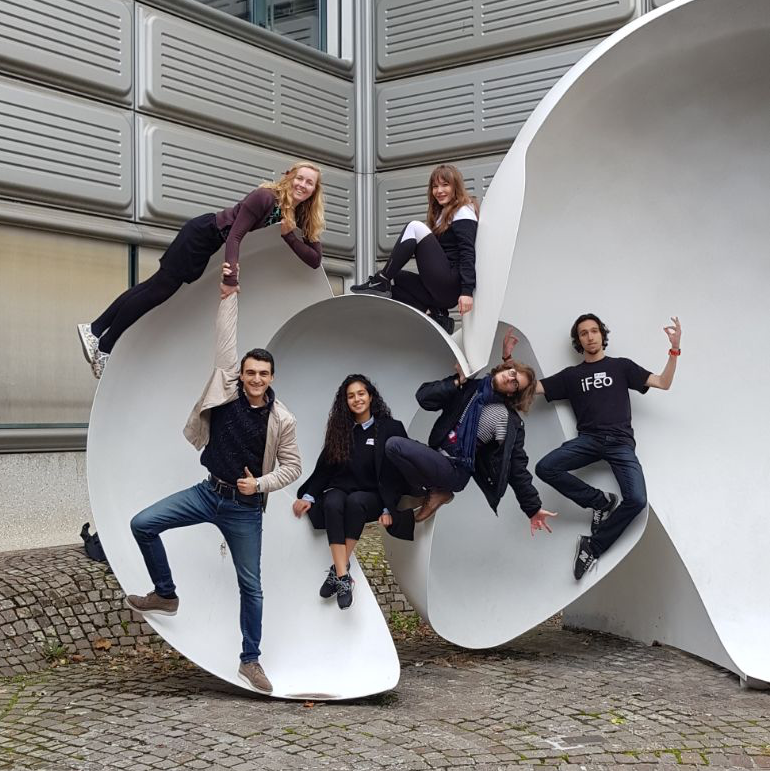
\includegraphics[scale=0.24]{images/CHIC.png}
    \caption{The NAPaC team with Chloe, Estelle, Simone, Marjane, Luca and Yann.}
    \label{fig:NAPaC_team}
\end{figure}



%%%%%%%%%%%%%%%%%%%%%%%%%%%%%%%%%%%%%%%%%% TERMINOLOGY %%%%%%%%%%%%%%%%%%%%%%%%%%%%%%%%%%%%%%%%%%%%%%%%%%%%%%%%%%%%%%
\newpage
\section{Terminology and Source files}

This section describes the main components of our prototype as well as the common expressions used throughout the report referring to them.

%\vspace{0cm}
%\begin{figure}[ht]
%    \centering
 %   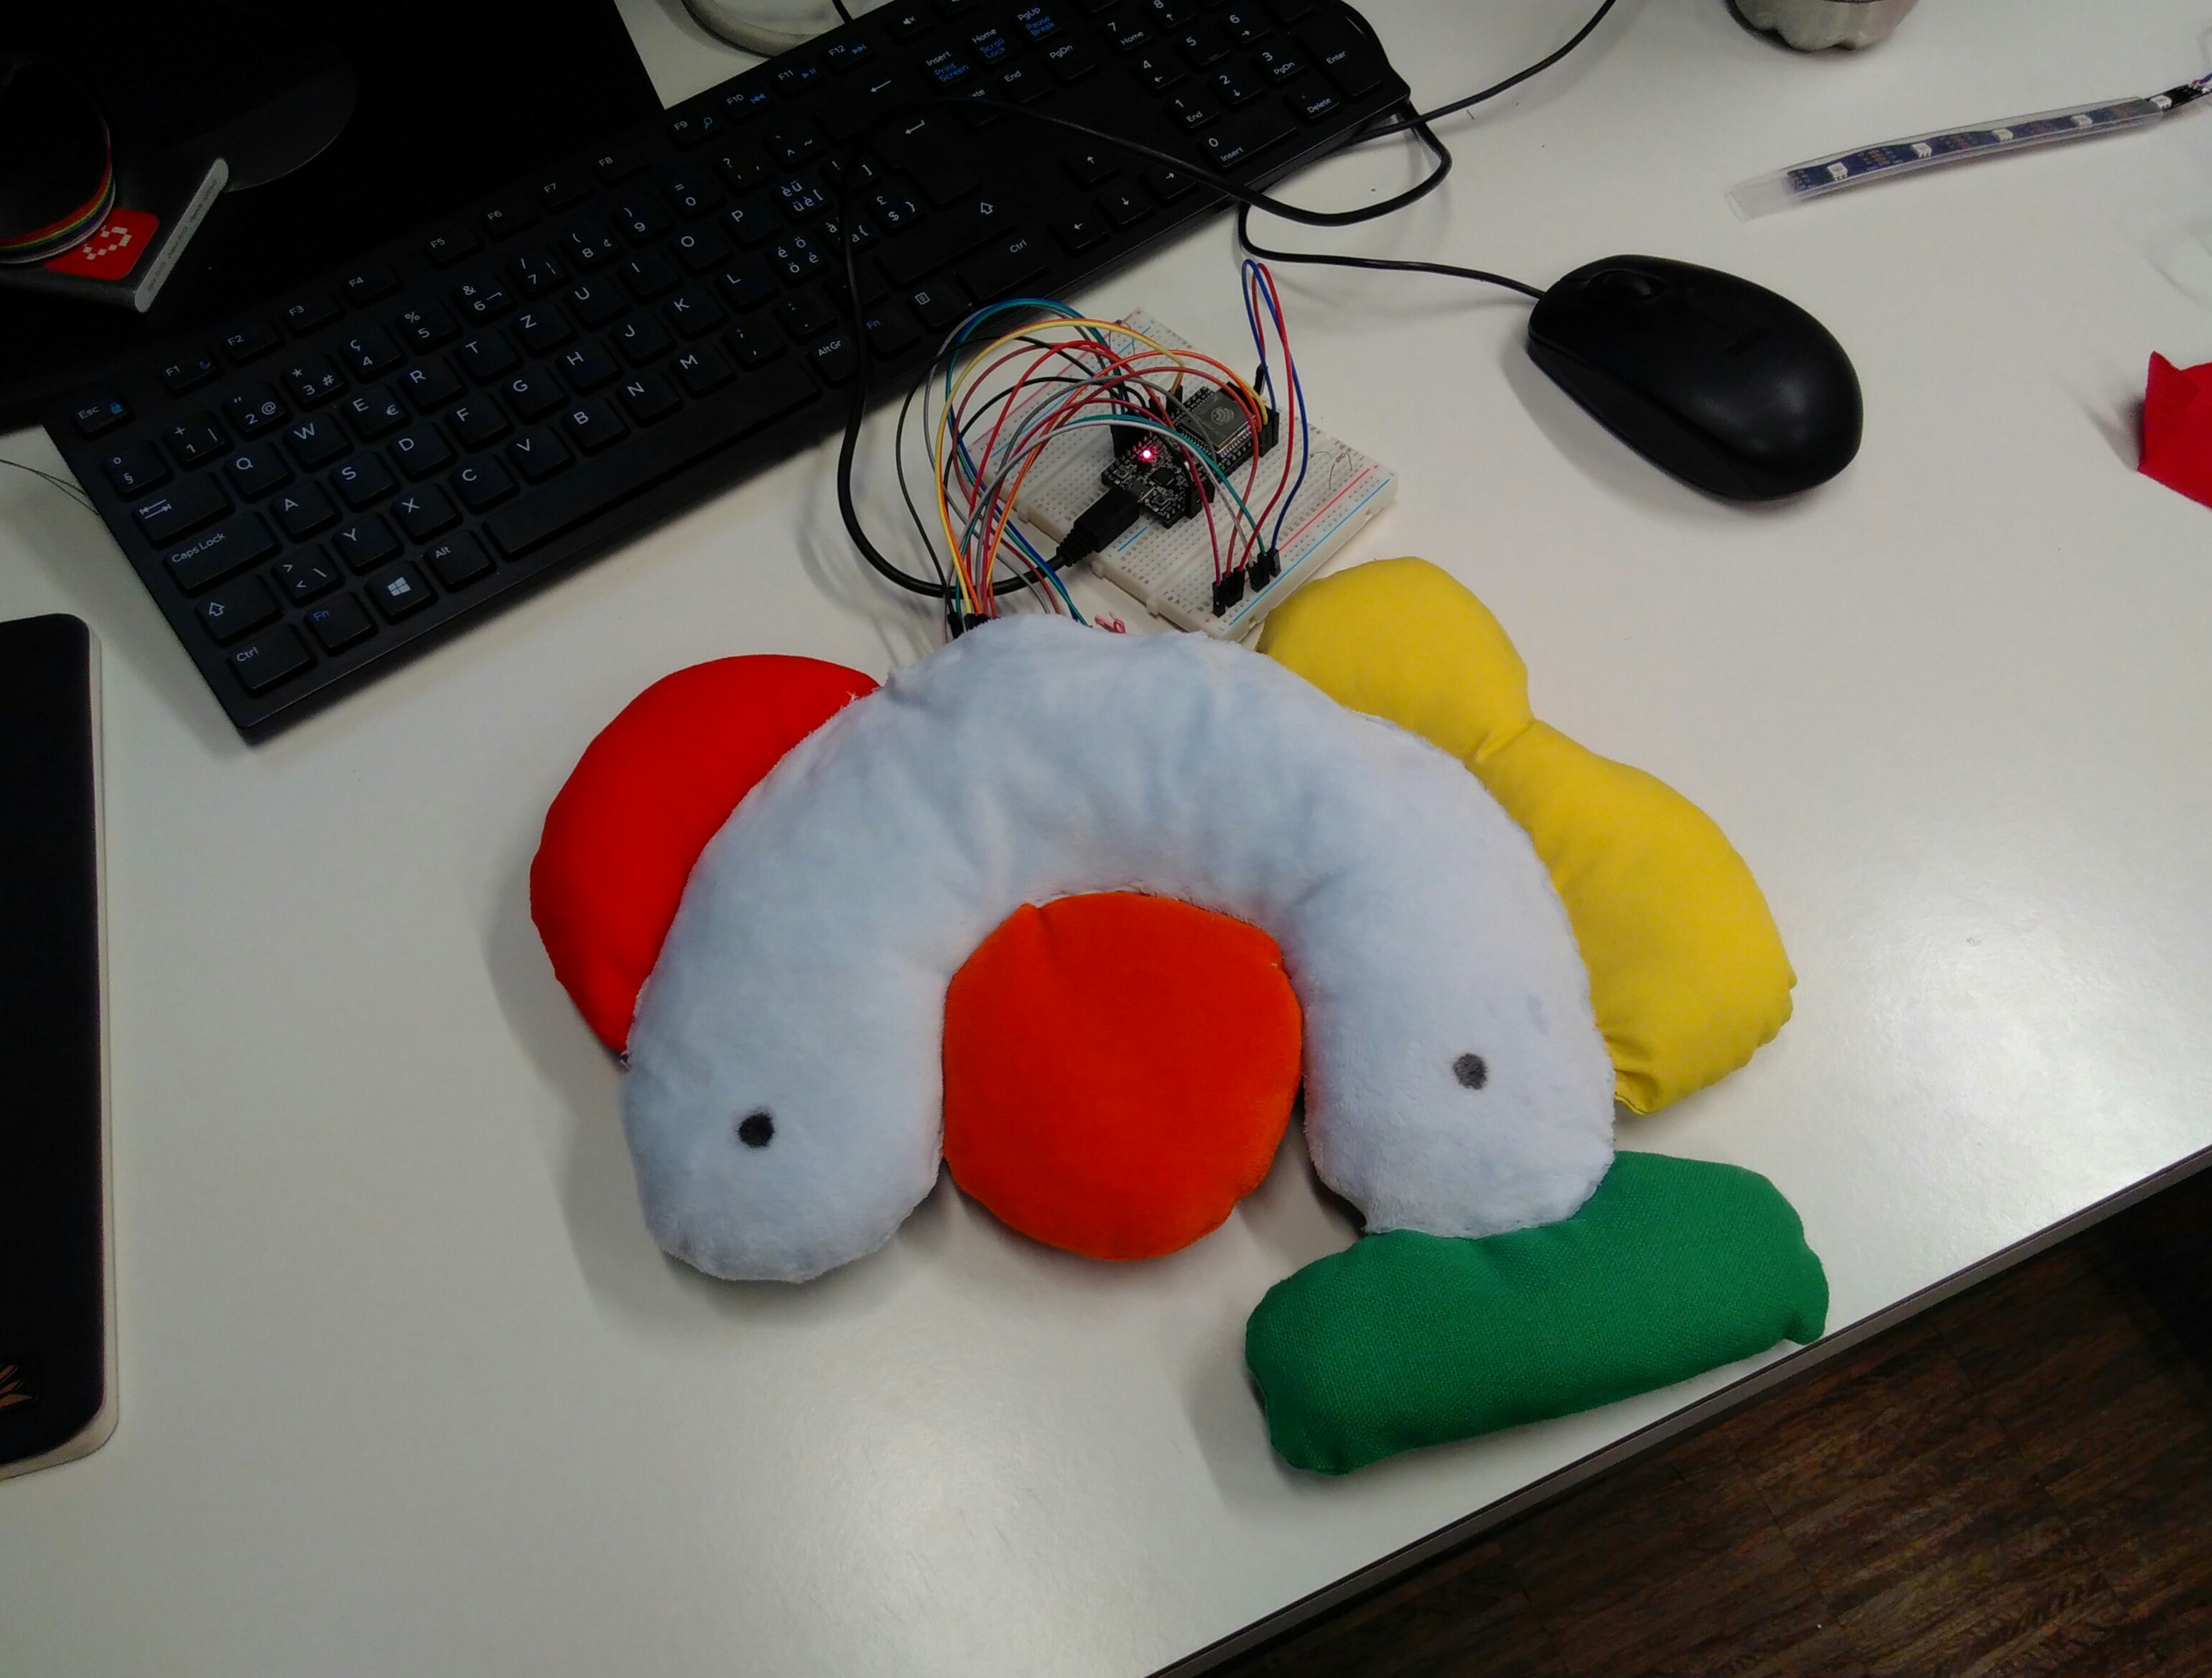
\includegraphics[width=0.5\textwidth]{images/HW/ms5.jpg}
  %  \caption{The plush toy prototype presented at MS5, with only the outer "Skin" visible}
   % \label{fig:proto_pic}
%\end{figure}

\begin{figure}[H]
    \centering
    \subfloat[Blackbox (or mechanical box)\label{fig:blackbox1}]{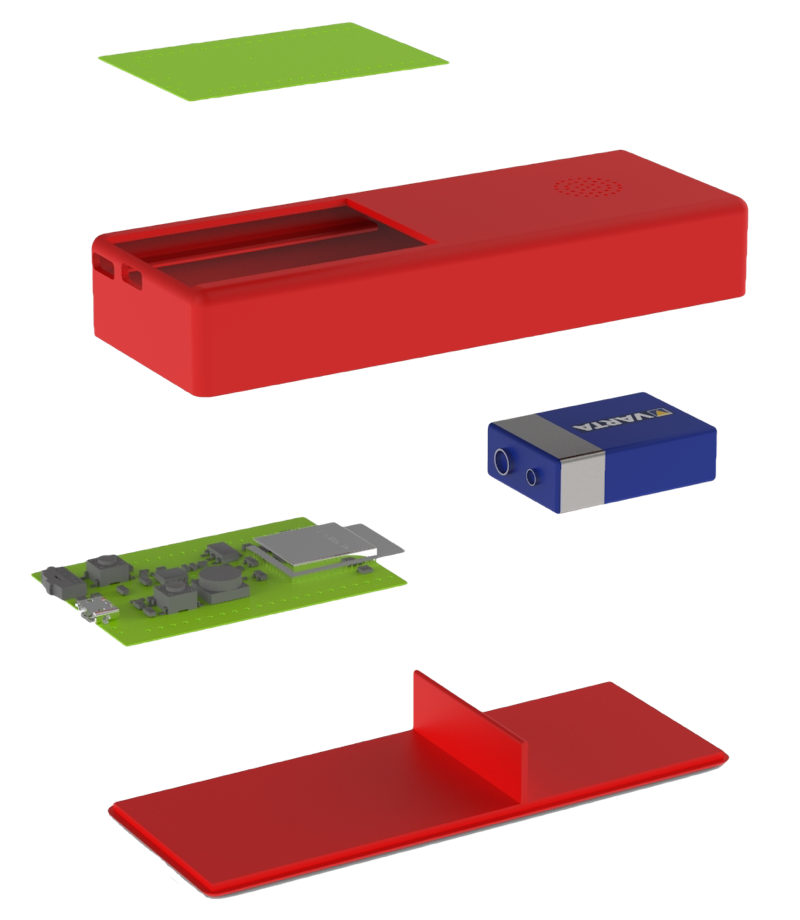
\includegraphics[width=0.3\textwidth]{images/HW/blackbox_v1.png}}\hfill
    \subfloat[Soft PCB\label{fig:softPCB1}] {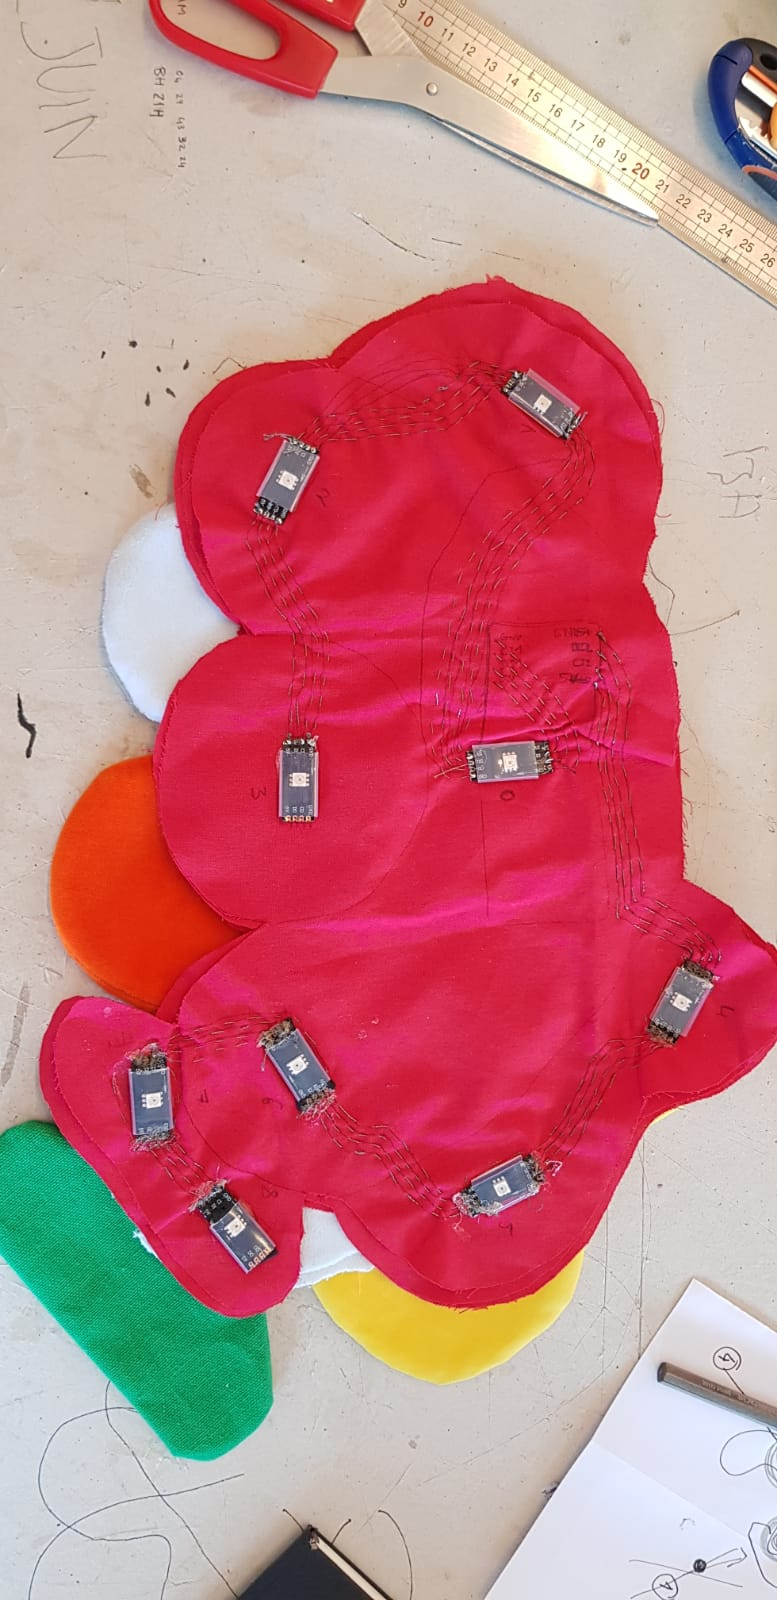
\includegraphics[width=0.3\textwidth, angle=90]{images/HW/softPCB_LEDs2.jpg}}\hfill
    \subfloat[Skin around soft PCB\label{fig:skin1}] {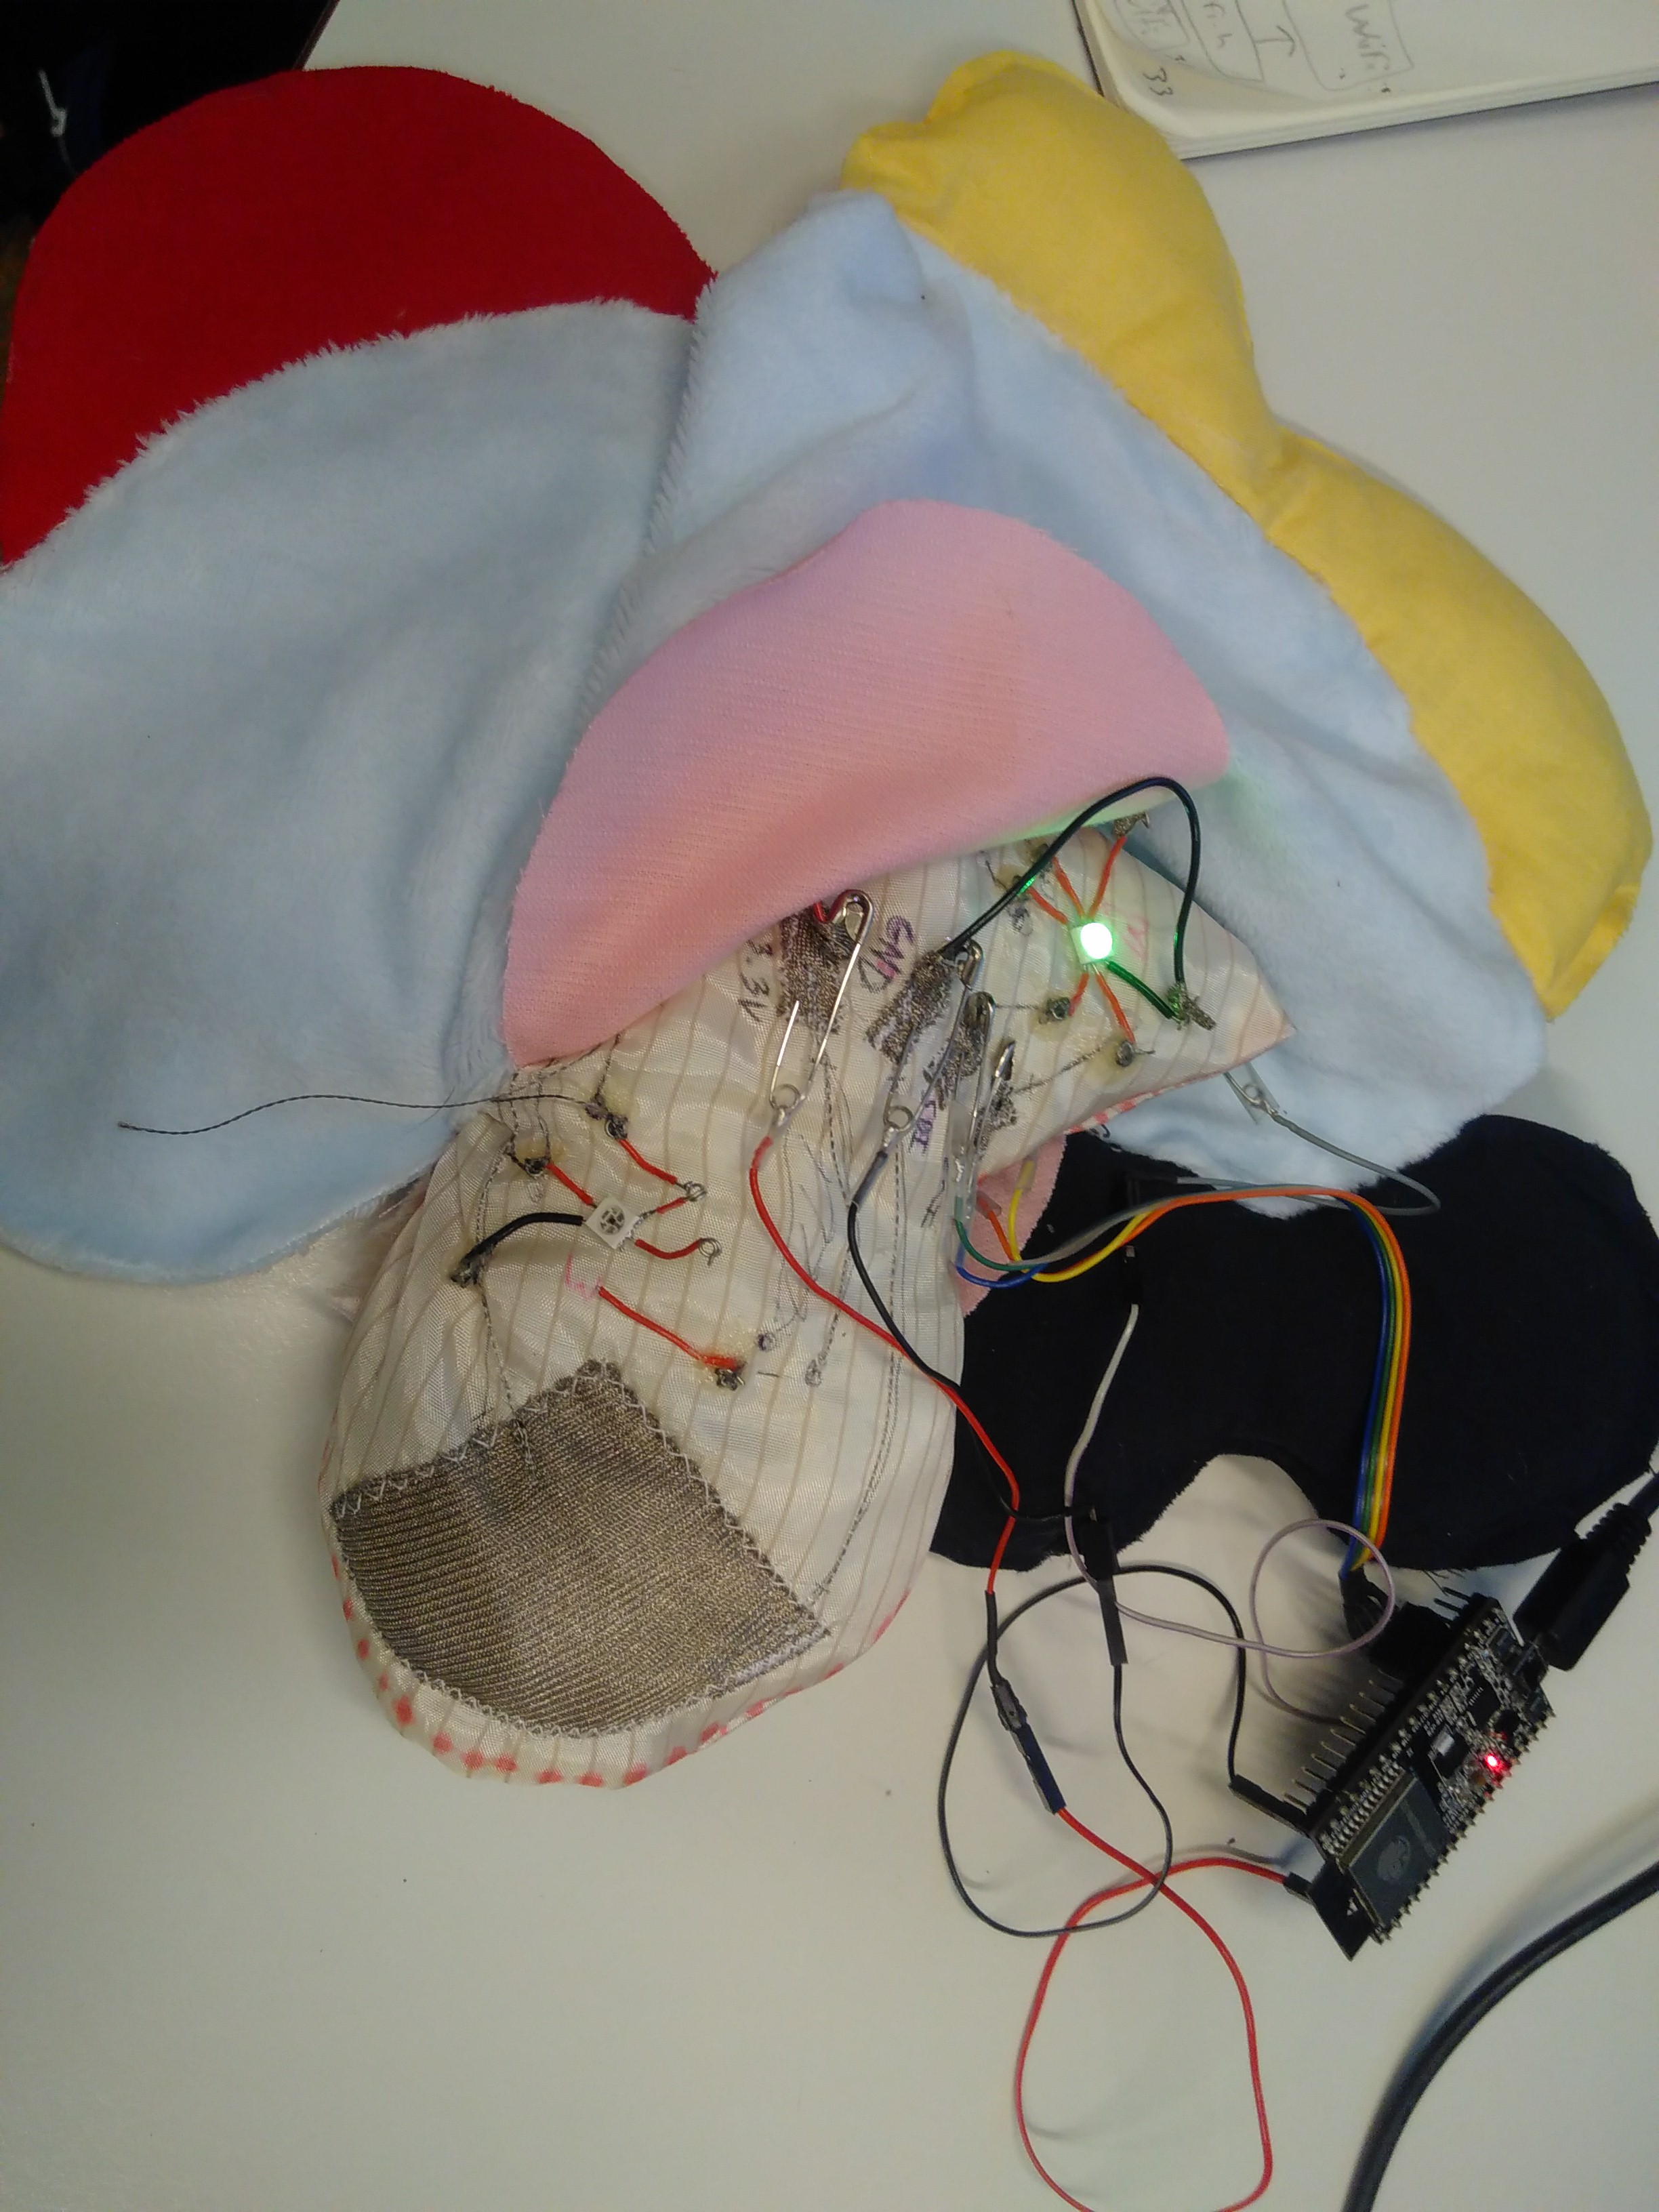
\includegraphics[width=0.3\textwidth, angle=90]{images/HW/proto1_connectors.jpg}}\hfill
    \caption{Main components of our prototype} 
    \label{fig:terminology}
\end{figure}



\begin{description}[align=left]
\item  [Blackbox (Fig. \ref{fig:blackbox1})] Inevitable "Hard" electronics such as microcontroller and battery, fitted in a slim housing inside of the plush toy. The blackbox is accessible through a zipper and can be removed for easy washing.
\item [Soft PCB (Fig. \ref{fig:softPCB1})] Textile electronics for interactions, such as LEDs and capacitive touch sensors, designed with conductive textile and threads to be soft and "invisible" to touch inside of the plush toy. The soft PCB connects to the blackbox and is fitted inside of the skin and soft stuffing.
\item [Skin (Fig. \ref{fig:skin1})] Soft textile layer surrounding all of the electronics, not taking into account any of the electronics components. This is the only part the child will interact with.
\end{description}

\subsection*{Github}

Our GitHub repository with all the files presented at MS5 (and illustrated in this report) can be found here: \url{https://github.com/mfeo15/CHIC-NAPaC}
